% Created 2021-05-13 Thu 01:02
% Intended LaTeX compiler: pdflatex
\documentclass[letter,12pt]{article}
\usepackage[utf8]{inputenc}
\usepackage[T1]{fontenc}
\usepackage{graphicx}
\usepackage{grffile}
\usepackage{longtable}
\usepackage{wrapfig}
\usepackage{rotating}
\usepackage[normalem]{ulem}
\usepackage{amsmath}
\usepackage{textcomp}
\usepackage{amssymb}
\usepackage{capt-of}
\usepackage{hyperref}
\usepackage[margin=1in]{geometry}
\usepackage[doublespacing]{setspace}
\usepackage{amsmath}
\usepackage{esvect}
\usepackage[round]{natbib}
\usepackage{authblk}
\hypersetup{colorlinks=true}
\author{Yousen Zhang}
\affil{Department of Physics and Astronomy, Rice University,\\ Houston, TX 77005, USA}
\date{\today}
\title{Gravitational lensing}
\hypersetup{
 pdfauthor={Yousen Zhang},
 pdftitle={Gravitational lensing},
 pdfkeywords={},
 pdfsubject={},
 pdfcreator={Emacs 27.2 (Org mode 9.4.4)}, 
 pdflang={English}}
\begin{document}

\maketitle

\begin{abstract}
Gravitational lensing effect was proposed in 1936 and finally observed in 1979. Besides the test of general relativity, it has become one of the most powerful techniques in astronomy, to probe dark matter and the geometry of the universe. In this paper, I will discuss the theoretical basics of the lensing effect and experimental results. These include the observation of the twin quasars, the application of gravitational lensing in determination of distributions of dark matter, and the measurements of Hubble constant.
\end{abstract}

\tableofcontents

\section{Introduction}
\label{sec:org82c717a}
\label{orgebbf9a4}
The general relativity is a theory of gravitation, established by
Einstein in 1915. It is a generalization of the special relativity,
in which theory the speed of light remains the same in all inertial
frames and the physical laws are expressed in covariant forms,
independent on the frames. In addition to the postulates above, two
additional principles are proposed in the general relativity. The
first one is that the inertial mass shows equivalence to the
gravitational mass. The effects from gravity can be effectively
eliminated in a small local region of space and time. In this sense,
physical laws seem the same as they are in flat space-time described
by Minkowskian space. The second principle is that the space-time is
curved rather than flat. The curvature is determined the gravity via
Einstein field equations.

Over the past century, the general relativity shows success through
the consistency with a lot of experiments. The perihelion precession
of planets are well described by Einstein's theory
\citep{RevModPhys.19.361}.  The precession of 42.88'' of Mercury's
orbit strongly supports the theory, for instance. The observation of
redshifts also shows the evidence of effects from the general
relativity. \cite{PhysRevLett.4.337} detected the energy loss of
\(\gamma\) ray at the receiver higher than the emitter, making use of
M\"{o}ssbauer effect. Recent observation of the gravitational
radiation shows great success of the theory of relativity as
well. LIGO collaboration announced the detection of the
gravitational waves from a binary black hole merger
\citep{Abbott:2016blz}.

Besides the phenomena mentioned above, an intriguing effects is the
deflection of light by a massive object. The light ray travels
along the geodesic which is not "straight" line anymore as a result
of curved space-time. This effect induce an interesting phenomena
called gravitational lensing, which was first proposed by
\cite{Einstein506}. If a massive object is placed between the source
and the observer, the light rays will be deflected and thus the
observer may find magnified images of the source. This phenomena was
confirmed by the discovery of quasar QSO 0957+561A,B
\cite{Walsh:1979nx}.

This paper will discuss the theoretical basics and experimental
results briefly. It is organized in the following way: simple models
of gravitational lensing will be introduced in Sec. \ref{org42febd1}; the
results in experiment will be discussed in Sec. \ref{org12600c4}; and
summary and outlook will be outlined in Sec. \ref{orgb7fedea}.

\section{Theoretical basics}
\label{sec:orgaf8760c}
\label{org42febd1}

In this section, a few simple models of gravitational lensing will
be discussed. Two categories will be introduced: lensing by the
point mass and lensing by the galaxy. Here we follow the
derivations in \cite{narayanlectures1997}.

In general, the mathematical formulism is hard to resolve and quite
complicated for the light propagation in an arbitrary curved
space. We limit ourselves in this paper by the weak gravitational
field and non-relativistic condition. Therefore the spacetime can be
described by a locally flat Minkowskian spacetime with perturbations
from the lensing object with Newtonian gravitational potential. The
motion of the mass object inducing lensing effect is also very slow.
These conditions are satisfied in most times. See discussions in
\cite{narayanlectures1997}.

\label{org97411f2} The light ray from distant source will be
deflected by an angle
\begin{equation}
  \vec{\hat{\alpha}} = \frac{4GM}{c^{2}b} \label{eq:alpha-hat}
\end{equation}
where M is the mass of lensing
  object and b is the impact parameter. The case considered here is
  limited that the both sources and observers are far away from the
  lensing. Thus the deflection happens in a very small region,
  characterized by the impact parameter. And the distribution along
  line of sight becomes unimportant. The intervening object can be
  treated as a thin sheet orthogonal to the line of sight. This plane
  of the mass sheet is usually referred to lens plane. The projected
  mass distribution, or surface mass distribution, is expressed by

  \begin{equation}
\Sigma(\vec{\xi}) = \int \rho(\vec{\xi}, z)dz \label{eq:mass-sheet}
  \end{equation}
where \(\vec{\xi}\) is the two-dimensional vector in the
lens plane. Combining \eqref{eq:alpha-hat} and \eqref{eq:mass-sheet}
will give the overall deflection by the thin mass sheet,
\begin{equation}
\vec{\hat{\alpha}} = \frac{4G}{c^2} \int \frac{(\vec{\xi}-\vec{\xi'})\Sigma(\vec{\xi'})}{|\vec{\xi}-\vec{\xi'}|^2} d^2 \xi'
\label{eq:alpha-mass-sum}
\end{equation}
For a circularly symmetric lens, as a special case, the problem is
reduced to one-dimension. The deflection angle is a function of the
distance to the center of the mass sheet in lens plane. The
expression is simplified as
\begin{equation}
\hat{\alpha} = \frac{4GM(\xi)}{c^2\xi}
\label{eq:alpha-mass-1D}
\end{equation}
where \(\xi\) is the distance from the lens center and M(\(\xi\)) is the
mass enclosed within the radius \(\xi\), given by
\begin{equation}
M(\xi) = 2\pi \int^{\xi}_0 \Sigma(\xi')\xi'd\xi'.
\label{eq:m-1D}
\end{equation}

\begin{figure}[htbp]
\centering
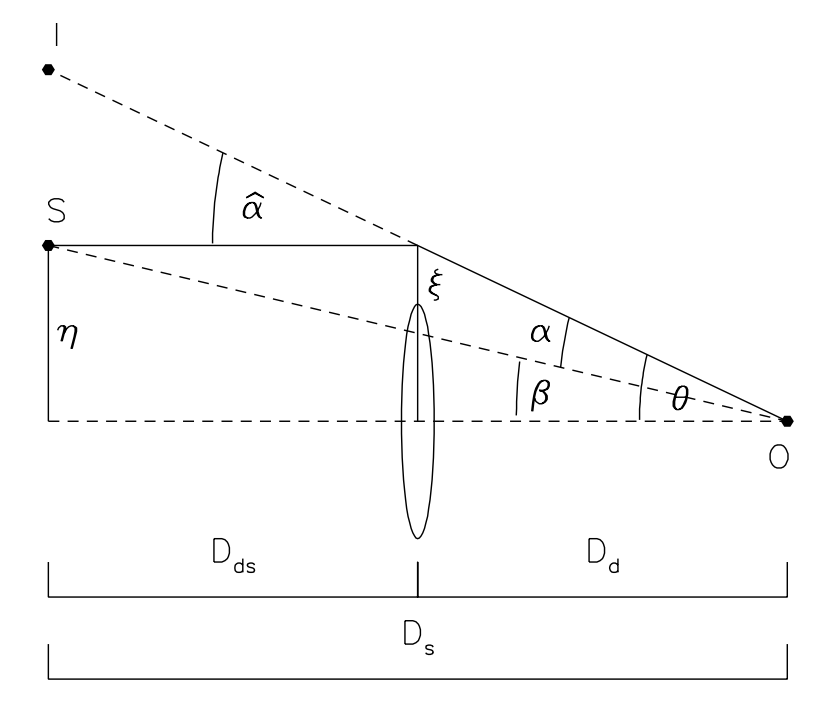
\includegraphics[width=.9\linewidth]{./figures/one_image.png}
\caption{\label{fig:org00b0bea}The illustration of lensing effect. The source, image and observer are denoted as S, I and O respectively. Credit: \cite{narayanlectures1997}.}
\end{figure}

As mentioned above, in the approximation of locally flat Minkowskian
spacetime with perturbations of gravitation, the relation
\begin{equation}
separation = distance \times angle \label{eq:distance}
\end{equation}
holds.  Denoting the distance between the observer and the source,
the observer and the lens, and the lens and the source with D\textsubscript{s}, D\textsubscript{d}
and D\textsubscript{ds}, respectively, we will have \(\theta D_s = \beta D_s -
  \hat{\alpha}D_{ds}\). This relation is obvious as illustrated in
Fig. \ref{fig:org00b0bea}.  Introducing reduced deflection angle
  \begin{equation}
\vec{\alpha} = \frac{D_{ds}}{D_s} \vec{\hat{\alpha}},
\label{eq:alpha-reduce}
  \end{equation}
lens equation is finally obtained
  \begin{equation}
\vec{\beta} = \vec{\theta} - \vec{\alpha}(\vec{\theta}). \label{eq:len}
  \end{equation}
Note that Equation \eqref{eq:distance} is not neccessary to be true in
curved space. However, Equations \eqref{eq:alpha-reduce} and
\eqref{eq:len} are true if the distance is \emph{defined} to satisfy the
Equation \eqref{eq:distance}.

Taking constant surface-mass density as an example, the reduced deflection angle is
  \begin{equation}
\alpha(\theta) = \frac{4\pi G\Sigma}{c^2}\frac{D_d D_{ds}}{D_s} \theta, \label{eq:alpha-reduce-circular}
  \end{equation}
setting \(\xi = D_d \theta\). For a lens lies on the optical axis
(\(\beta\)=0), the corresponding constant surface mass density is
\begin{equation}
\Sigma_{cr} = \frac{c^2}{4\pi G} \frac{D_s}{D_d D_{ds}}. \label{eq:sigma-critical}
\end{equation}
The light rays from the sources perfectly focus on the position of
observer, though the focus length depends on both the lensing object
and the positions of the source and the observer. In this case, the
mass density is referred as \emph{critical} surface mass density. In case
of \(\Sigma\) > \(\Sigma\)\textsubscript{cr}, multiple images will show up and the
corresponding surface mass density is referred as \emph{supercritical}.

Considering the case of the circularly symmetric lens, but with an
arbitraty mass distribution, according to Equations \eqref{eq:alpha-hat}
and \eqref{eq:alpha-reduce}, the lens equation becomes
\begin{equation}
\beta(\theta) = \theta - \frac{D_{ds}}{D_d D_s} \frac{4GM(\theta)}{c^2\theta} \label{eq:len-circular}.
\end{equation}
For a source lying on the optic axis (\(\beta\)=0) the solution for the images reads
   \begin{equation}
\theta_E = \bigg[ \frac{4GM(\theta_E)}{c^2} \frac{D_{ds}}{D_d D_s}\bigg]^{1/2}
   \end{equation}
From the rotational symmetry, we know that the images are located
at the ring of \(\theta\)\textsubscript{E}. The ring is called Einstein ring and the
\(\theta\)\textsubscript{E} is called Einstein radius.

An instructive example is the case of lensing by point mass, the Einstein radius is given by
   \begin{equation}
\theta_E = \bigg[ \frac{4GM}{c^2} \frac{D_{ds}}{D_d D_s}\bigg]^{1/2}
   \end{equation}
and the lens equation reads
   \begin{equation}
\beta = \theta - \frac{\theta_E^2}{\theta}.
   \end{equation}
The images are
\begin{equation}
\theta_{\pm} = \frac{1}{2} \bigg( \beta\pm\sqrt{\beta^2+4\theta_E^2} \bigg).
\end{equation}
Thus one is inside the Einstein ring and the other is outside.

Though the phenomena is intersting, the magnification of point
mass lens is hard to observe unless the lens is extremely
massive. However, the detection become reliable if the lens and the
source move relative to each other. The relative motion will enlarge
the lensing-induced time delay and the effect is referred as
microlensing if the lensing object has stellar mass. And it has been
observed in QSO 2237+0305 \citep{1990ApJ_358L_33W}.

\label{org6b0629e} The point mass model has been discussed so
far. It turns out complicated and dependent on the model of mass
distribution when considering galaxies as lens. Here we consider a
simple model.

We assume the constituents in the galaxies behave like particles of
ideal gas. Their gravitational potential is spherical symmetric and
confining them inside the galaxy. The equation of state of these
mass constituents reads
   \begin{equation}
p = \frac{\rho kT}{m} \label{eq:thermal-energy}
   \end{equation}
where \(\rho\) is the mass density of the galaxy and the m is the mass
of the constituent. In thermal equilibrium, we have
   \begin{equation}
\frac{1}{2} m \sigma_{v}^2 = \frac{1}{2} kT
   \end{equation}
where \(\sigma\)\textsubscript{v} is the one-dimensional velocity dispersion. Assuming
the galaxy is isothermal, the dispersion is constant over the
region of the galaxy. The hydrostatic equation
\(\frac{\nabla p}{\rho}=\vec{f}\) reads
\begin{equation}
\frac{1}{\rho} \frac{dp}{dr} = -\frac{GM(r)}{r^2} \label{eq:hydrostatic}
\end{equation}
since \(\rho\), p and M are merely functions of r and \(\frac{dM}{dr} =
  4\pi r^2 \rho\) due to the rotational symmetry. Combing Equations
\eqref{eq:thermal-energy} and \eqref{eq:hydrostatic}, the solution reads
\begin{equation}
\rho(r) = \frac{\sigma_v^2}{2\pi G}\frac{1}{r^2}.
\end{equation}

This mass distribution is referred as the \emph{singular isothermal
sphere}. The density is proportional to r\textsuperscript{-2}. There are also other
models for the mass distribution of galaxies but we will not discuss
them here.

It is also useful to define the the projected Newtonian potential of
the lens. It is related to the magnification of the lens. The projected
potential is defined as
\begin{equation}
\psi(\vec{\theta}) = \frac{D_{ds}}{D_d D_s} \frac{2}{c^2} \int \Phi(D_d \vec{\theta}, z)dz
\end{equation}
where \(\Phi\) is the Newtonian in three-dimension. The gradient of \(\psi\)
with respect to \(\theta\) is simply \(\vec{\alpha}\),
\begin{equation}
\nabla_{\theta} \psi = \vec{\alpha}.
\end{equation}
And we know the divergence of the gravitational potential is
proportional to the mass density. Thus we have
\begin{equation}
\nabla^2_{\theta} \psi = \frac{2}{c^2} \frac{D_d D_{ds}}{D_s} \int \nabla^2_\xi \Phi dz = \frac{2}{c^2}\frac{D_d D_{ds}}{D_s} 4\pi G\Sigma = 2\frac{\Sigma(\vec{\theta})}{\Sigma_{cr}}\equiv 2\kappa(\vec{\theta}).
\end{equation}
The term \(\kappa\) is called convergence.

The magnification of the lens is defined as
\begin{equation}
magnification = \frac{image\,\, area}{source\,\, area} = \mathrm{det}( \frac{\delta \theta^2} {{\delta \beta^2}} ).
\end{equation}
Thus the Jacobian matrix \(A\equiv\partial\vec{\beta}/\partial\vec{\theta}\)
is the inverse of the magnification tensor. We have
\begin{equation}
A = \bigg(\delta_{ij} - \partial{\alpha_i}/\partial \beta_j\bigg) = \bigg( \delta_{ij} - \frac{\partial^2\psi}{\partial\theta_i\theta_j} \bigg).
\end{equation}
It can be further written as
\begin{align}
\begin{split}
A &=
\begin{pmatrix}
1-\kappa-\gamma_1 & -\gamma_2 \\
-\gamma_2 & 1+\kappa+\gamma_1
\end{pmatrix}
\\
&=(1-\kappa)
\begin{pmatrix}
1 & 0\\0 & 1
\end{pmatrix}
-\gamma
\begin{pmatrix}
\cos{2\phi} & \sin{2\phi} \\
\sin{2\phi} & -\cos{2\phi}
\end{pmatrix},
\end{split}
\end{align}
by introducing notations
\begin{align}
\frac{\partial^2\psi}{\partial\theta_i\theta_j} &\equiv \psi_{ij} \\
\kappa &= \frac{1}{2}(\psi_{11}+\psi_{22}) \\
\gamma_1 &= \frac{1}{2}(\psi_{11}-\psi_{22})\equiv \gamma \cos{2\phi} \\
\gamma_2 &= \psi_{12} = \psi_{21} \equiv \gamma \sin{2\phi}.
\end{align}
Term \(\kappa\) is named convergence and \(\gamma\)\textsubscript{j} is named shear
tensor. The quantity \(\gamma\) denotes the magnitude of the shear and
\(\phi\) denotes the orientation. The magnification is
\begin{equation}
\mathrm{det}A^{-1} = \frac{1}{(1-\kappa)^2-\gamma^2}.
\end{equation}

\section{Experimental results}
\label{sec:org0423fba}
\begin{figure}[htbp]
\centering
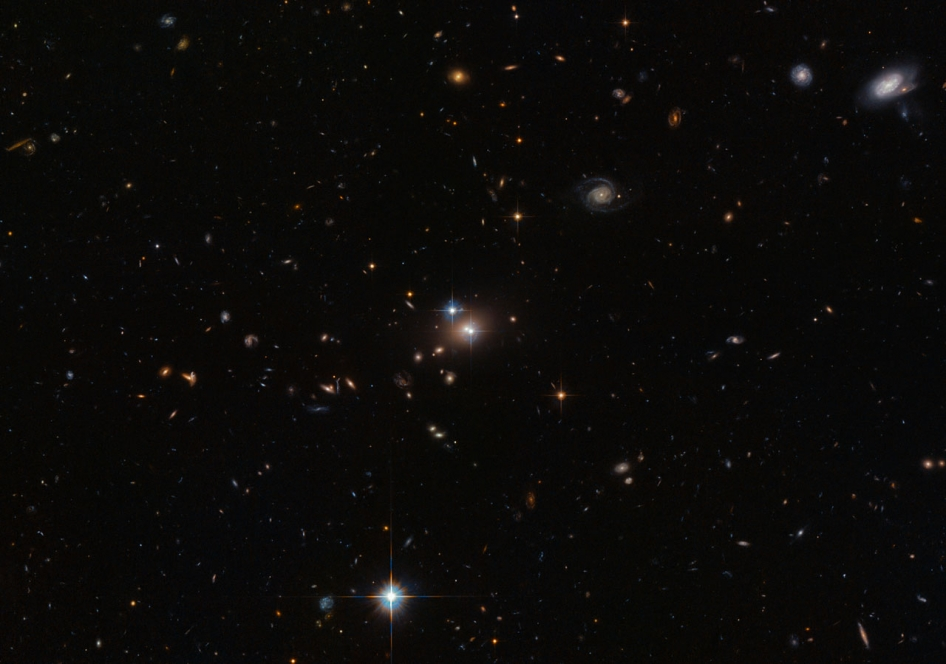
\includegraphics[width=.9\linewidth]{./figures/twin.jpg}
\caption{\label{fig:org43fbdc0}Quasar QSO09567+561. Credit: Hubble Space Telescope.}
\end{figure}

\label{org12600c4} As mentioned in Sec. \ref{orgebbf9a4}, the discovery of
QSO957+561A,B shows strong evidence of the existence of
gravitational lensing effect \citep{Walsh:1979nx}. Fig. \ref{fig:org43fbdc0}
shows the image of the quasar QSO957+561 by Hubble Space Telescope.
The results are briefly discussed here. QSO957+561A,B are images of
a single quasar. A quasar is also known as a quasi-stellar object
(QSO), discovered by \cite{schmidt3c1963}. It is the nuclear region
with extremely high luminosity of a remote galaxy. As a result of
large distance, the probability of observing lensing effects of
massive objects between quasars and observers become large. Quasars
provide opportunities to discover gravitational lensing in
experiments. The explanation of lensing effects for two images,
QSO957+561A,B, separated by 6'', was finally confirmed by
\cite{1980ApJ241507Y,1984ApJ287538G}. Fig. \ref{fig:orgd1d859c}
show the spectra of wavelength of QSO957+561A,B and they show
similarity with each other. The evidence is provided by the facts
below:
\begin{itemize}
\item The similarity of flux spectra between two images.
\item The intervening galaxy between images and the observers
\item The luminous distribution of cores of two images are related by a
magnification matrix according to lensing effects.
\end{itemize}

\begin{figure}[htbp]
\centering
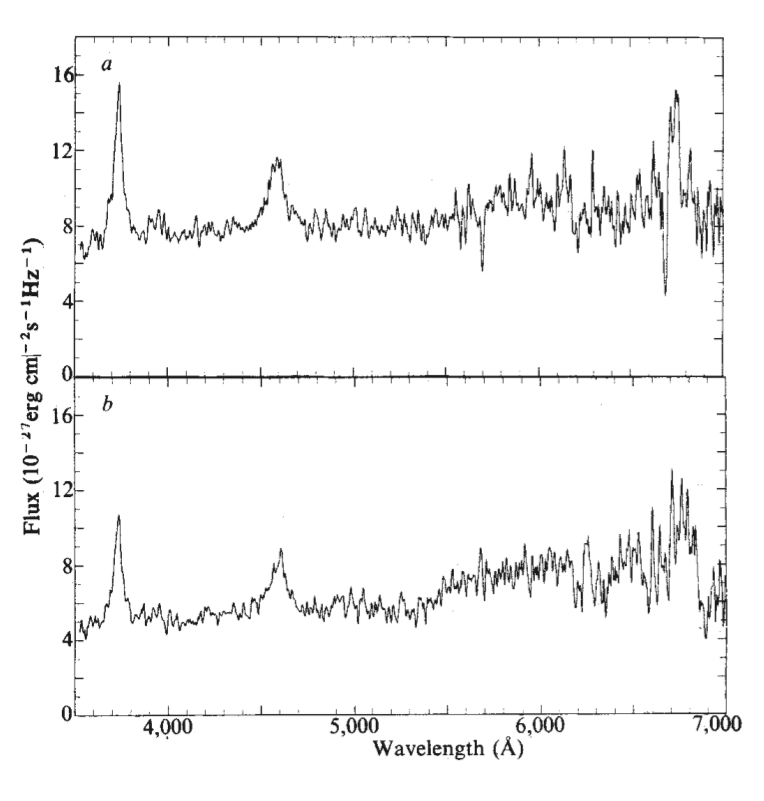
\includegraphics[width=.9\linewidth]{./figures/QuasarsAB.png}
\caption{\label{fig:orgd1d859c}The spectra of wave length of QSO0957+561A,B \citep{Walsh:1979nx}. The upper pannel (a) is for image A and lower one (b) is for B.}
\end{figure}

In addition to the test of gravitation theory, the lensing effects
can also help in several ways in the astronomical measurements. It
was proposed that the Hubble constant could be measured through the
gravitational lensing \citep{1964MNRAS128307R}. The time of light
propagation of two images are uneven since the effective length of
path are different. The time delay difference \(\Delta \tau\) between two
images is proportional to the difference of path of length and thus
the inverse of Hubble constant (H\textsubscript{0}\textsuperscript{-1}). The product
\(H_0\Delta\tau\) depends merely on the geometric positions of
sources, lensing and observers and the model of lensing
effects. Once \(H_0\Delta\tau\) is determined and \(\Delta \tau\) is
measured, the Hubble constant is also obtained.

The way using gravitational lensing to determine Hubble constant has
several advantages \citep{narayanlectures1997}:
\begin{itemize}
\item The sources are distant at large redshifts and their velocities
can be considered small enough compared to the Hubble flow.
\item The measurements does not wait for the motion of sources with the
expansion of the universe. There is no need to measure the
increasing distance and time interval. The time delay of images
can be measured in a short time.
\item The gravitational lensing originates the general relativity, which
is well tested in a series of experiments. It is less
model-dependent or less empirical.
\end{itemize}

To precisely measure the Hubble constant, several difficulties need
to be overcome. These include: the precision measurements of the
differences between arrival times of multiple images; the
understanding of the distortion of the angular diameter distances
along the line of sight; the model for the mass distribution of the
lens \citep{Birrer2020}. The procedures of time delay measurements has
been validated via simulations \citep{2015ApJ_799_168D}. The
distortion of line of sight is corrected statistically via
comparisons with numerical simulations \citep{2011MNRAS_410_2167F} and
the residual is negligible compared to overall uncertainties
\citep{Millon_2020}. The third issue is still under investigation. One
recent measurement implementing gravitational lensing infers that
the the value of Hubble constant is \(73.3^{+1.7}_{1.8}\) km s\textsuperscript{-1}
Mpc\textsuperscript{-1}, in agreement with local measurements type Ia supernovae
\citep{Wong2019}. Fig. \ref{fig:orgc7a4d76} shows the probability density
distribution of H\textsubscript{0}.

\begin{figure}[htbp]
\centering
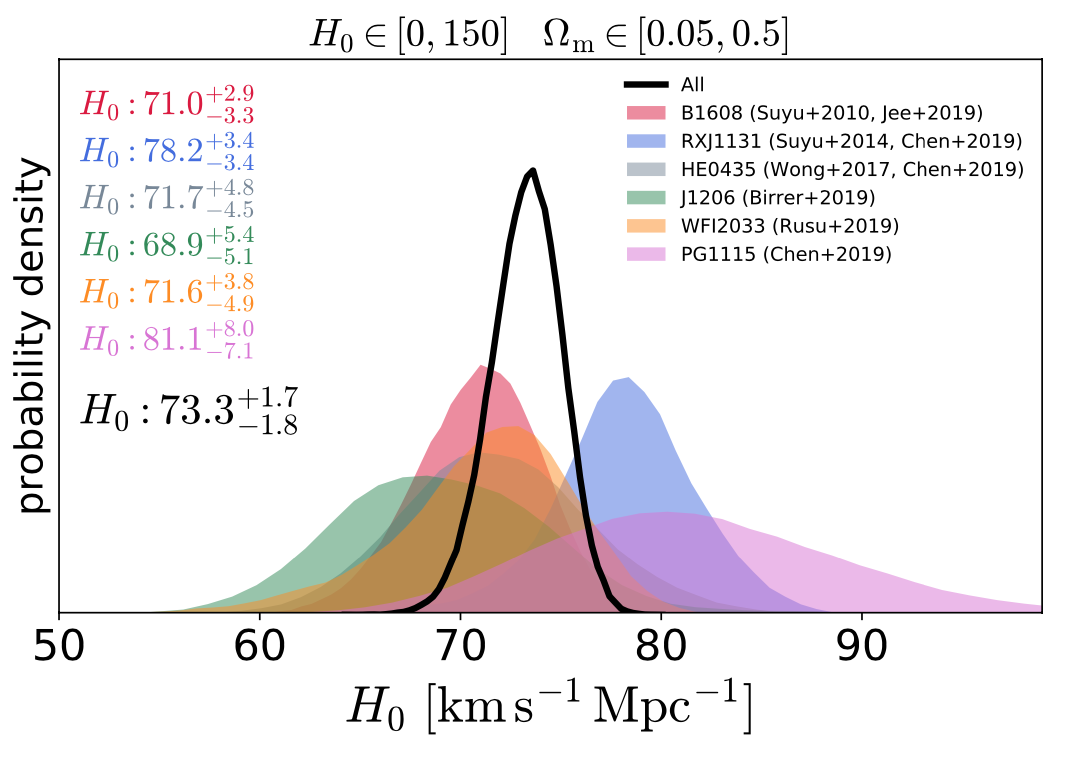
\includegraphics[width=.9\linewidth]{./figures/H0WongEtAl.png}
\caption{\label{fig:orgc7a4d76}The posterior probability density distributions for H\textsubscript{0} from different individual lensing systems. Six systems are denoted by shaded area and the black curve is the combined result of H\textsubscript{0} \citep{Wong2019}.}
\end{figure}

Besides the implication for Hubble constant, gravitational lensing
also serve as powerful tools to probe the lensing objects
themselves. Thus it provide good probes to searching for dark matter
and dark energy. And it merely depends on the mass distributions of
dark matters, regardless the their intrinsic nature.

However, several issues presents in the processes of exploration of
dark matters. Signals from large-scale structure is very faint with
little chance to detect. And mass distributions of measurable
galaxies are need to be fixed as priori. The atmosphere of the Earth
also smears the signal. To overcome these difficulties, Hubble Space
Telescope was launched. It produced the projected 2D map of dark
matters for the fist time \citep{Massey2007}. Fig. \ref{fig:orgce62878}
shows the comparison between the distributions of dark matters and
ordinary matters. The similarity between maps of dark matters and
maps of baryonic matters indicates that dark matters are still under
the rule of gravitation \citep{Ellis2010darkmatter}.

\begin{figure}[htbp]
\centering
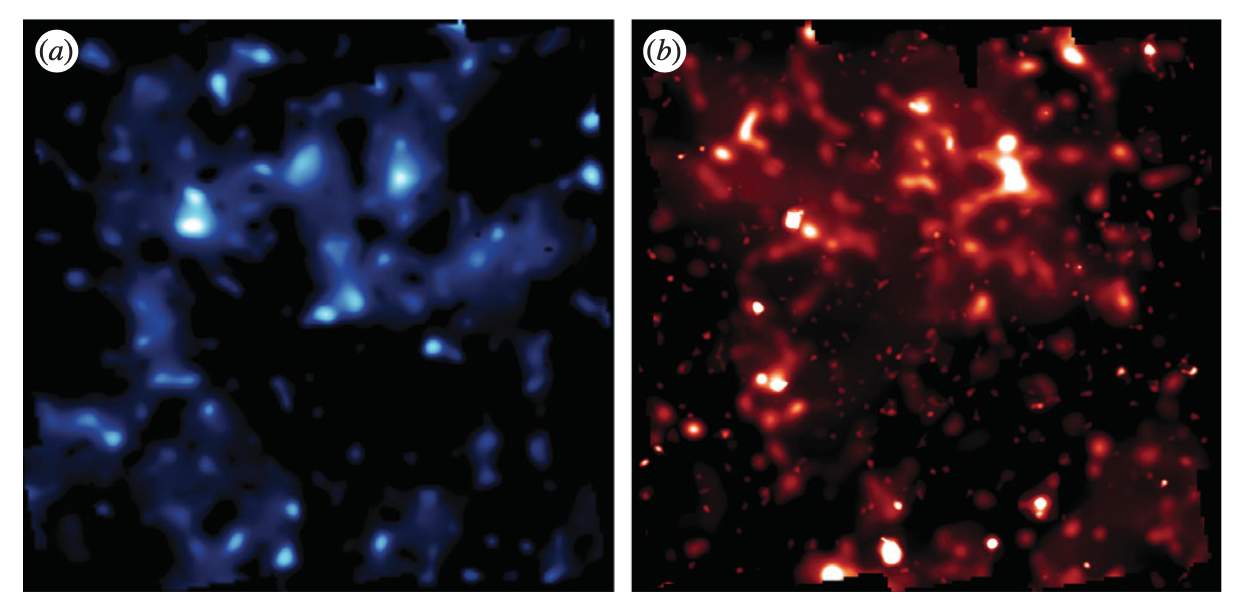
\includegraphics[width=.9\linewidth]{./figures/dark_matter.png}
\caption{\label{fig:orgce62878}The projected distribution of dark matters and baryonic matters. (a) The blue maps the density distribution of dark matter \citep{Massey2007}. (b) Equivalent map of baryonic matter. Credit: Hubble Space Telescope}
\end{figure}

In addition to the studies of dark matters in cluster, the search
for dark matters in a galaxy is also of interests. The gravitational
effects assist to detect the haloes of a galaxy. Measurements are
performed via galaxy-galaxy lensing, selecting a subset of
classified images. Combing these images will give the average
density of dark matter of a given galaxy.

\section{Summary and outlook}
\label{sec:orgc0728c7}
\label{orgb7fedea} The theoretical basics and experimental outputs have
been presented in this paper. The gravitational lensing as a
manifestation of Einstein's theory have been observed in many
experiments. In addition to serving merely tests for the theory of
gravitation, the lensing effects have advantages for astronomical
observations. It helps in several aspects: detecting the distant
objects which is invisible without lensing effects; probing the mass
distribution of the lensing objects, for instance, dark matters;
determining the overall properties of the universe. These
measurements have enriched the knowledge for the universe and
provide valuable experiences to explore further.

\begin{figure}[htbp]
\centering
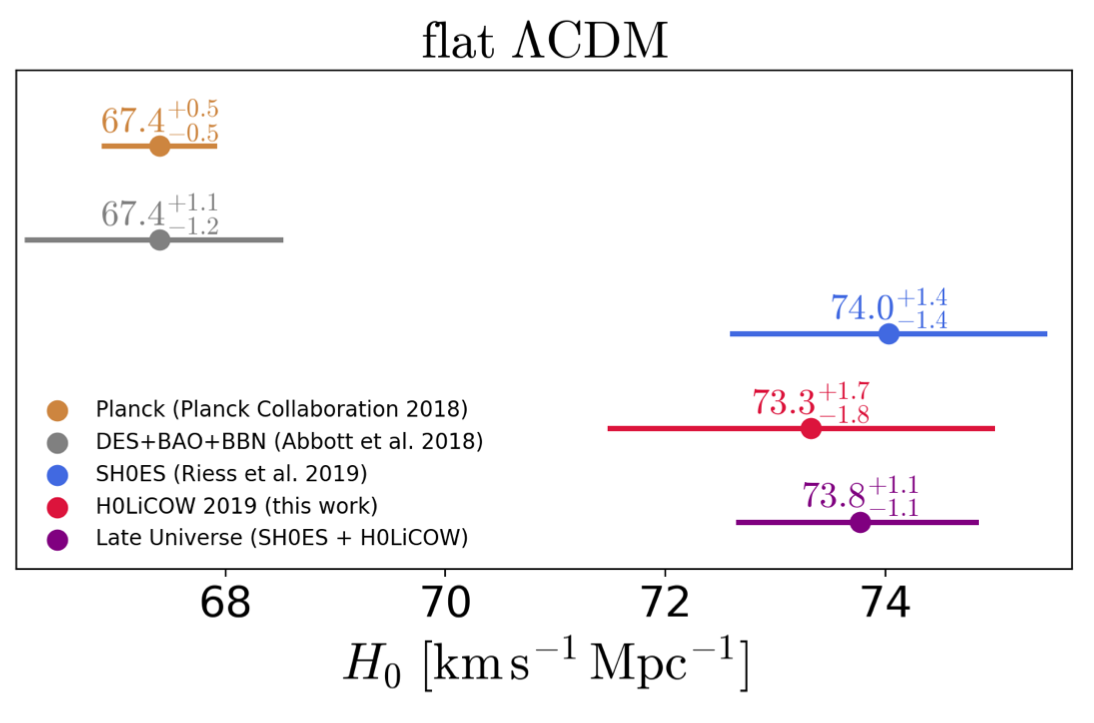
\includegraphics[width=.9\linewidth]{./figures/H0discrepancy.png}
\caption{\label{fig:orgcaf3856}H\textsubscript{0} values from different experiments \citep{Planck2018results,Abbott_2018,Riess_2019,Wong2019}.}
\end{figure}

The recent measurements of Hubble constant shows discrepancy between
the early universe value from cosmic micro waves and late universe
value from gravitational lensing with a tension of \(5.3\sigma\)
\citep{Wong2019}. This raise a question whether there is new physics
behind the puzzle. Before proposing new physics theories, further
constraints on the cosmography of time delay are needed at
first. The precision of H\textsubscript{0} values by gravitational lensing can be
further improved.

There are also discrepancies between the standard cold dark mater
(CDM) paradigm and observations. \cite{Meneghetti_2020} reported an
excess of more than an order of magnitude of gravitational lensing
than the predictions from CDM simulations. Either the unresolved
systematic issues with simulations or the correction to CDM model
are needed to explain the results.

In summary, gravitational lensing manifest itself the evidence of
general relativity. It is also valuable probe to explore the
universe. More interesting physics phenomena can be explored in the
future, using the lensing technique.

\bibliographystyle{abbrvnat}
\bibliography{refs}
\end{document}
